\section{Auswertung}
\label{sec:Auswertung}
\subsection{Messung im Niederdruckbereich bis 1 bar} % (fold)
\label{sub:Niederdruck_aus}


\begin{figure}
  \centering
  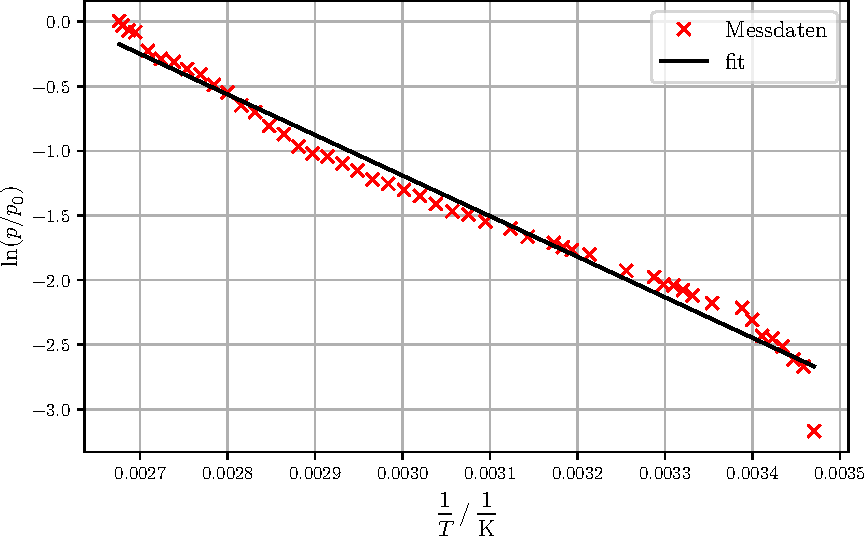
\includegraphics[scale=0.7]{build/plot1.pdf}
  \caption{Messwerte und Ausgleichsgerade im Niederdruckbereich bis 1 bar.}
  \label{fig:plot1}
\end{figure}

a = -3139.3111660225786 ± 69.52967119503401
b = 8.227105045902752 ± 0.21329983575246847
L = (2.61+/-0.06)e+04
La= 3101.122
Li= (2.30+/-0.06)e+04
Li in eV = 0.238+/-0.006

\subsection{Messung im Hochdruckbereich von 1 bis 15 bar} % (fold)
\label{sub:Hochdruck_aus}


\begin{figure}
  \centering
  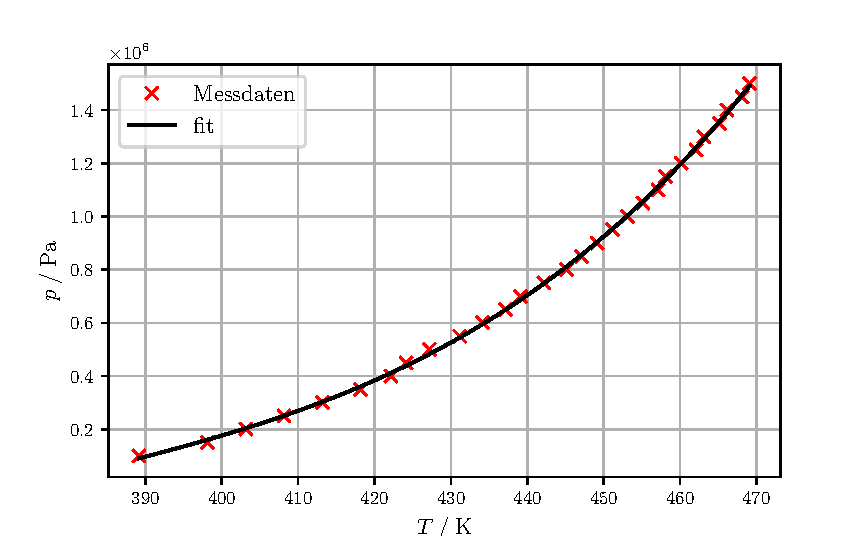
\includegraphics[scale=0.7]{build/plot2.pdf}
  \caption{Messwerte und Ausgleichsgerade im Hochdruckbereich von 1 bis 15 bar.}
  \label{fig:plot2}
\end{figure}
\begin{align*}
  a = 1.2008796738162035 ± 0.16199747636566664\\
  b = -1371.9346764297973 ± 209.5543809877098\\
  c = 529627.3673322977 ± 90215.5596509826\\
  d = -69021623.98027332 ± 12925631.459950624
\end{align*}

\begin{figure}[htbp]
  \begin{subfigure}{\textwidth}
  \centering
  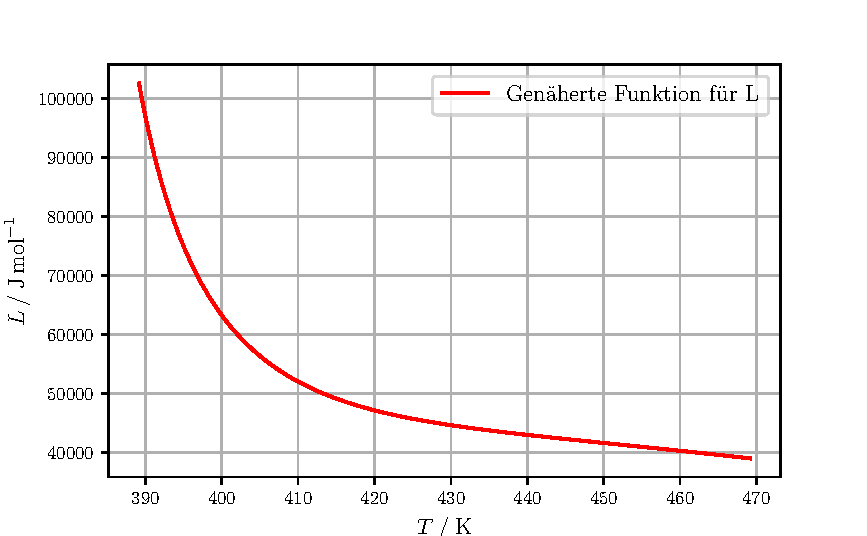
\includegraphics[scale=0.7]{build/plot3.pdf}
  \caption{positive Wurzel.}
  \label{fig:plot3}
\end{subfigure}
\begin{subfigure}{\textwidth}
  \centering
  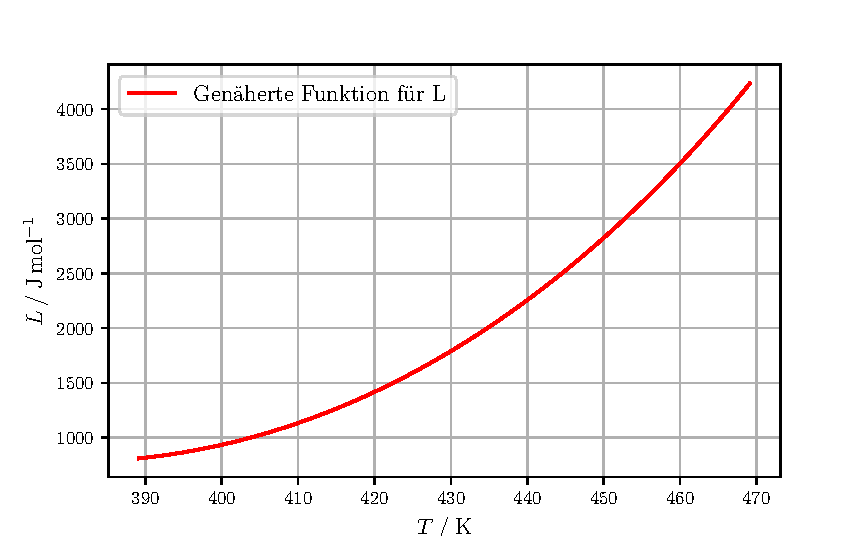
\includegraphics[scale=0.7]{build/plot4.pdf}
  \caption{negative Wurzel.}
  \label{fig:plot4}
\end{subfigure}
\end{figure}

